\documentclass[]{article}
\usepackage[left=1in,top=1in,right=1in,bottom=1in]{geometry}


%%%% more monte %%%%
\usepackage{wrapfig}
% thispagestyle{empty}
% https://stackoverflow.com/questions/2166557/how-to-hide-the-page-number-in-latex-on-first-page-of-a-chapter
\usepackage{color}
% \usepackage[table]{xcolor} % are they using color?

% \definecolor{WSU.crimson}{HTML}{981e32}
% \definecolor{WSU.gray}{HTML}{5e6a71}

% \definecolor{shadecolor}{RGB}{248,248,248}
\definecolor{WSU.crimson}{RGB}{152,30,50} % use http://colors.mshaffer.com to convert from 981e32
\definecolor{WSU.gray}{RGB}{94,106,113}

%%%%%%%%%%%%%%%%%%%%%%%%%%%%

\newcommand*{\authorfont}{\fontfamily{phv}\selectfont}
\usepackage{lmodern}


  \usepackage[T1]{fontenc}
  \usepackage[utf8]{inputenc}




\usepackage{abstract}
\renewcommand{\abstractname}{}    % clear the title
\renewcommand{\absnamepos}{empty} % originally center

\renewenvironment{abstract}
 {{%
    \setlength{\leftmargin}{0mm}
    \setlength{\rightmargin}{\leftmargin}%
  }%
  \relax}
 {\endlist}

\makeatletter
\def\@maketitle{%
  \pagestyle{empty}
  \newpage
%  \null
%  \vskip 2em%
%  \begin{center}%
  \let \footnote \thanks
    {\fontsize{18}{20}\selectfont\raggedright  \setlength{\parindent}{0pt} \@title \par}%
}
%\fi
\makeatother









\title{\textbf{\textcolor{WSU.crimson}{Denzel Washington is Better Than
Will Smith}} \newline \textbf{\textcolor{WSU.gray}{An Analysis of the
Career of Denzel Washington vs Will Smith}}  }
 

%  

% \author{ \Large true \hfill \normalsize \emph{} }
\author{\Large Peyton
Urquhart\vspace{0.05in} \newline\normalsize\emph{Student of Software
Engineering (WSU)}  }


\date{April 26, 2021}
\setcounter{secnumdepth}{3}

\usepackage{titlesec}
% See the link above: KOMA classes are not compatible with titlesec any more. Sorry.
% https://github.com/jbezos/titlesec/issues/11
\titleformat*{\section}{\bfseries}
\titleformat*{\subsection}{\bfseries\itshape}
\titleformat*{\subsubsection}{\itshape}
\titleformat*{\paragraph}{\itshape}
\titleformat*{\subparagraph}{\itshape}

% https://code.usgs.gov/usgs/norock/irvine_k/ip-092225/


%\titleformat*{\section}{\normalsize\bfseries}
%\titleformat*{\subsection}{\normalsize\itshape}
%\titleformat*{\subsubsection}{\normalsize\itshape}
%\titleformat*{\paragraph}{\normalsize\itshape}
%\titleformat*{\subparagraph}{\normalsize\itshape}

% https://tex.stackexchange.com/questions/233866/one-column-multicol-environment#233904
\usepackage{environ}
\NewEnviron{auxmulticols}[1]{%
  \ifnum#1<2\relax% Fewer than 2 columns
    %\vspace{-\baselineskip}% Possible vertical correction
    \BODY
  \else% More than 1 column
    \begin{multicols}{#1}
      \BODY
    \end{multicols}%
  \fi
}





\usepackage{natbib}
\setcitestyle{aysep={}} %% no year, comma just year
% \usepackage[numbers]{natbib}
\bibliographystyle{./../../latex-setup/biblio/ormsv080.bst}



\usepackage[strings]{underscore} % protect underscores in most circumstances




\newtheorem{hypothesis}{Hypothesis}
\usepackage{setspace}


%%%%%%%%%%%%%%%%%%%%%%%%%%%%%%%%%%%%%%%%%%%%%%%%%%%%%
%%% MONTE ADDS %%%

\usepackage{fancyhdr} % fancy header 
\usepackage{lastpage} % last page 

\usepackage{multicol}


\usepackage{etoolbox}
\AtBeginEnvironment{quote}{\singlespacing\small}
% https://tex.stackexchange.com/questions/325695/how-to-style-blockquote


\usepackage{soul}			%% allows strike-through
\usepackage{url}			%% fixes underscores in urls
\usepackage{csquotes}		%% allows \textquote in references
\usepackage{rotating}		%% allows table and box rotation
\usepackage{caption}		%% customize caption information
\usepackage{booktabs}		%% enhance table/tabular environment
\usepackage{tabularx}		%% width attributes updates tabular
\usepackage{enumerate}		%% special item environment
\usepackage{enumitem}		%% special item environment

\usepackage{lineno}		%% allows linenumbers for editing using \linenumbers
\usepackage{hanging}


\usepackage{mathtools}  	%% also loads amsmath
\usepackage{bm}		%% bold-math
\usepackage{scalerel}	%% scale one element (make one beta bigger font)

\newcommand{\gFrac}[2]{ \genfrac{}{}{0pt}{1}{{#1}}{#2} }

\newcommand{\betaSH}[3]{  \gFrac{\text{\tiny #1}}{{\text{\tiny #2}}}\hat{\beta}_{\text{#3}}   }
\newcommand{\betaSB}[3]{              ^{\text{#1}} _{\text{#2}} \bm{\beta} _{\text{#3}}                   }  %% bold
\newcommand{\bigEQ}{  \scaleobj{1.5}{{\ }= } }
\newcommand{\bigP}[1]{  \scaleobj{1.5}{#1 } }





\usepackage{endnotes}  % he already does this ...
\renewcommand{\enotesize}{\normalsize}
% https://tex.stackexchange.com/questions/99984/endnotes-do-not-be-superscript-and-add-a-space
\renewcommand\makeenmark{\textsuperscript{[\theenmark]}} % in brackets %
% https://tex.stackexchange.com/questions/31574/how-to-control-the-indent-in-endnotes
\patchcmd{\enoteformat}{1.8em}{0pt}{}{}

\patchcmd{\theendnotes}
  {\makeatletter}
  {\makeatletter\renewcommand\makeenmark{\textbf{[\theenmark]} }}
  {}{}



% https://tex.stackexchange.com/questions/141906/configuring-footnote-position-and-spacing

\addtolength{\footnotesep}{5mm} % change to 1mm

\renewcommand{\thefootnote}{\textbf{\arabic{footnote}}}
\let\footnote=\endnote
%\renewcommand*{\theendnote}{\alph{endnote}}
%\renewcommand{\theendnote}{\textbf{\arabic{endnote}}}


\renewcommand*{\notesname}{}

\makeatletter
\def\enoteheading{\section*{\notesname
  \@mkboth{\MakeUppercase{\notesname}}{\MakeUppercase{\notesname}}}%
  \mbox{}\par\vskip-2.3\baselineskip\noindent\rule{.5\textwidth}{0.4pt}\par\vskip\baselineskip}
\makeatother


\renewcommand*{\contentsname}{}

\renewcommand*{\refname}{REFERENCES}


%\usepackage{subfigure}
\usepackage{subcaption}

\captionsetup{labelfont=bf}  % Make Table / Figure bold

%%% you could add elements here ... monte says .... %%%
%\usepackage{mypackageForCapitalH}


%%%%%%%%%%%%%%%%%%%%%%%%%%%%%%%%%%%%%%%%%%%%%%%%%%%%%

% set default figure placement to htbp
\makeatletter
\def\fps@figure{htbp}
\makeatother


% move the hyperref stuff down here, after header-includes, to allow for - \usepackage{hyperref}

\makeatletter
\@ifpackageloaded{hyperref}{}{%
\ifxetex
  \PassOptionsToPackage{hyphens}{url}\usepackage[setpagesize=false, % page size defined by xetex
              unicode=false, % unicode breaks when used with xetex
              xetex]{hyperref}
\else
  \PassOptionsToPackage{hyphens}{url}\usepackage[draft,unicode=true]{hyperref}
\fi
}

\@ifpackageloaded{color}{
    \PassOptionsToPackage{usenames,dvipsnames}{color}
}{%
    \usepackage[usenames,dvipsnames]{color}
}
\makeatother
\hypersetup{breaklinks=true,
            bookmarks=true,
            pdfauthor={Peyton Urquhart (Student of Software Engineering
(WSU))},
             pdfkeywords = {data analytics; data science;},  
            pdftitle={Denzel Washington is Better Than Will Smith: An
Analysis of the Career of Denzel Washington vs Will Smith},
            colorlinks=true,
            citecolor=blue,
            urlcolor=blue,
            linkcolor=magenta,
            pdfborder={0 0 0}}
\urlstyle{same}  % don't use monospace font for urls

% Add an option for endnotes. -----

%
% add tightlist ----------
\providecommand{\tightlist}{%
\setlength{\itemsep}{0pt}\setlength{\parskip}{0pt}}

% add some other packages ----------

% \usepackage{multicol}
% This should regulate where figures float
% See: https://tex.stackexchange.com/questions/2275/keeping-tables-figures-close-to-where-they-are-mentioned
\usepackage[section]{placeins}



\pagestyle{fancy}   
\lhead{\textcolor{WSU.crimson}{\textbf{ Denzel Washington is Better Than
Will Smith }}}
\chead{}
\rhead{\textcolor{WSU.gray}{\textbf{  Page\ \thepage\ of\ \protect\pageref{LastPage} }}}
\lfoot{}
\cfoot{}
\rfoot{}


\begin{document}
	
% \pagenumbering{arabic}% resets `page` counter to 1 
%    

% \maketitle

{% \usefont{T1}{pnc}{m}{n}
\setlength{\parindent}{0pt}
\thispagestyle{plain}
{\fontsize{18}{20}\selectfont\raggedright 
\maketitle  % title \par  

}

{
   \vskip 13.5pt\relax \normalsize\fontsize{11}{12} 
   
\textbf{\authorfont Peyton Urquhart} \hskip 15pt \emph{\small Student of
Software Engineering (WSU)}   

}

}








\begin{abstract}

    \hbox{\vrule height .2pt width 39.14pc}

    \vskip 8.5pt % \small 

\noindent Data from IMDB is analyzed for actors Will Smith and Denzel
Washington. This report aims to portray Denzel Washington as a better
overall actor than Will Smith. The angle I took for this report was to
analyze critic ratings across genres for the actors. Audience ratings
are also briefly covered.


\vskip 8.5pt \noindent \textbf{\underline{Keywords}:} data analytics;
data science; \par

    




    
    \hbox{\vrule height .2pt width 39.14pc}
    \vskip 5pt 
    \hfill \textbf{\textcolor{WSU.gray}{ April 26, 2021 } }
    \vskip 5pt 
    
\end{abstract}


\vskip -8.5pt



 % removetitleabstract

\noindent  

\begin{figure}[!ht]
 \label{fig:one-graphic}
%% figures have hrule, tables have hline
    \begin{center}
        \scalebox{1.00}{    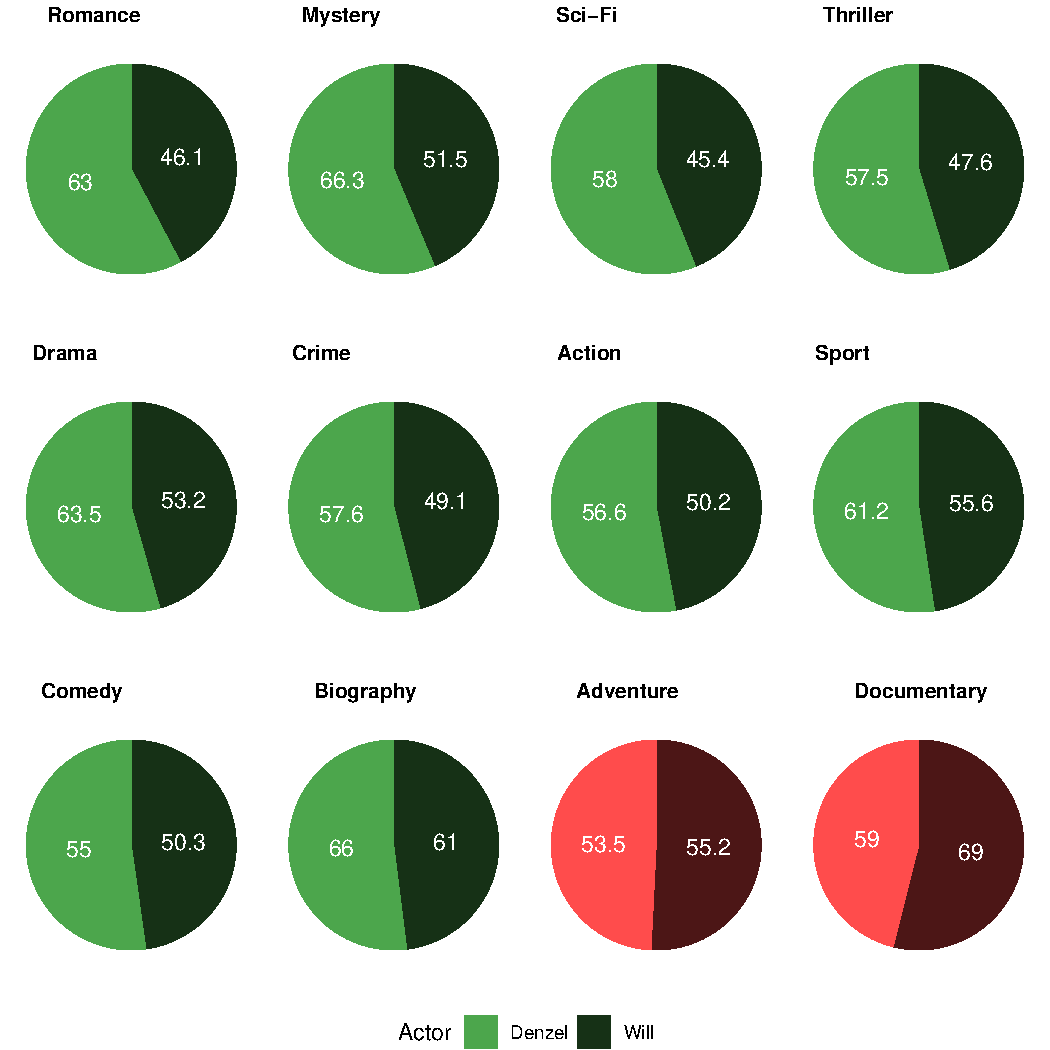
\includegraphics{figures/1graphic.pdf} }
    \end{center}
    \hrule
      \vspace{2mm}
    \caption{ \textbf{Average Critic Ratings Across Genres:} \newline \footnotesize{ Displayed above are average critic ratings across movie genres for Will Smith and Denzel Washington's 60 most popular movies. This graphic omits genres for which one or both of the actors do not have available data, such as "Animation" for Denzel Washington. \newline \newline Displayed in green are genres where Denzel out-performs Will, the contrary is displayed in red.}  }
    \vspace{2mm}
    \hrule
\end{figure}

\section{Commentary}
\label{sec:commentary}
\doublespacing

\noindent Denzel Washington has higher critic ratings on average in
10/12 of the genres which are common among Will and himself. Included in
these ``green genres'' are the most popular genres among the two actors:
Action and Comedy. \newline

\noindent Will out-performs Denzel in the Adventure genre by only a
small margin of 0.3/100. Additionally, the genre where Will is found to
perform much better, documentaries, could hardly be considered acting in
the first place. \newline

\begin{figure}[!ht]
 \label{fig:one-graphic}
%% figures have hrule, tables have hline
    \begin{center}
        \scalebox{1.00}{    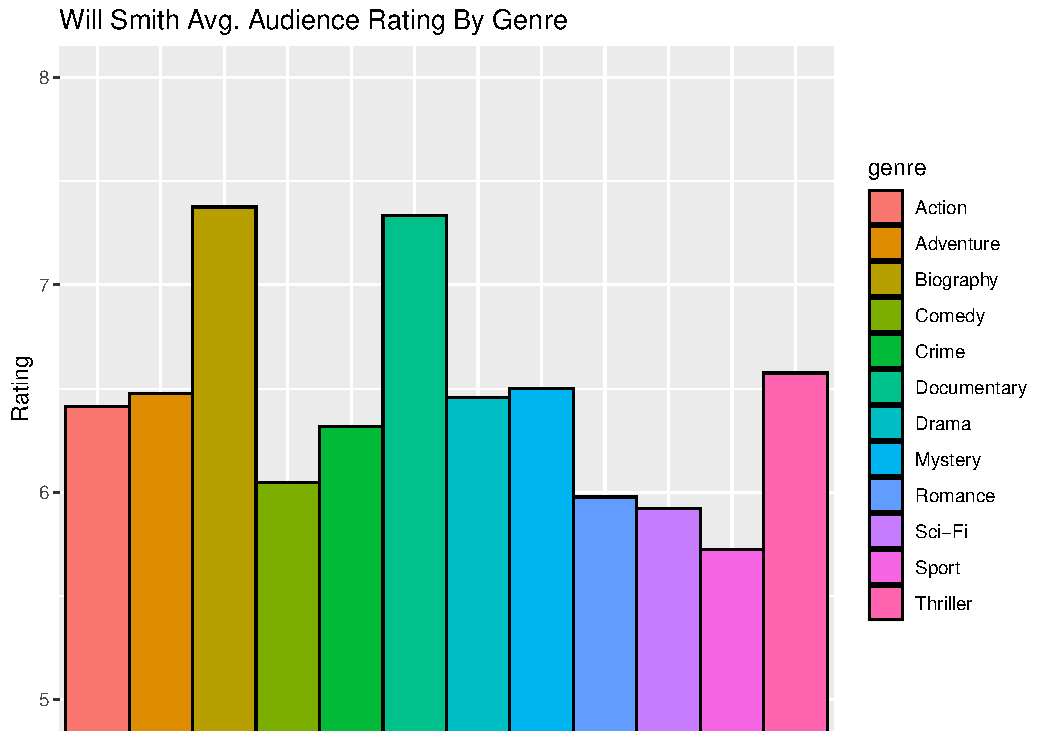
\includegraphics{figures/will-avg-aud.pdf} }
    \end{center}
    \hrule
      \vspace{2mm}
    \caption{ \textbf{Will Smith: Average Audience Rating by Genre:} \newline \footnotesize{ Displayed above is Will Smith's average audience rating (1-10) by movie genre. This graphic omits genres for which one or both of the actors do not have available data}  }
    \vspace{2mm}
    \hrule
\end{figure}

\begin{figure}[!ht]
 \label{fig:one-graphic}
%% figures have hrule, tables have hline
    \begin{center}
        \scalebox{1.00}{    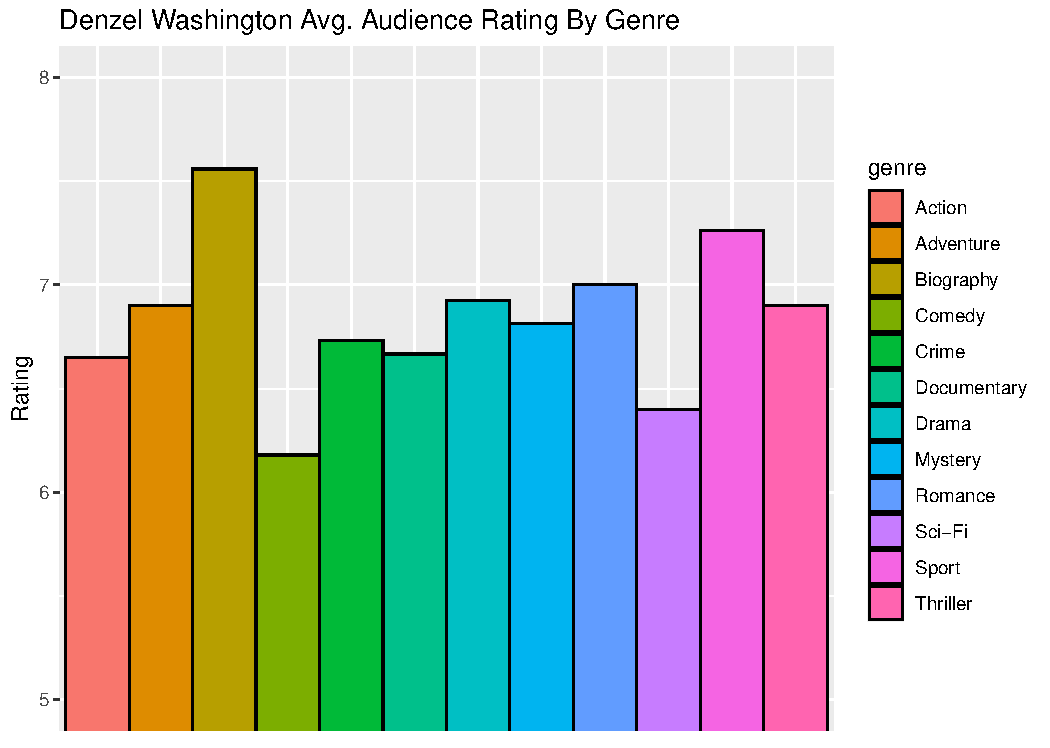
\includegraphics{figures/denzel-avg-aud.pdf} }
    \end{center}
    \hrule
      \vspace{2mm}
    \caption{ \textbf{Denzel Washington: Average Audience Rating by Genre:} \newline \footnotesize{ Displayed above is Denzel Washingtons's average audience rating (1-10) by movie genre. This graphic omits genres for which one or both of the actors do not have available data}  }
    \vspace{2mm}
    \hrule
\end{figure}

\section{Commentary}
\label{sec:commentary}
\doublespacing

\noindent In addition to Denzel achieving much higher critic-ratings in
general, he also recieved much stronger ratings from the audience.
\newline

\noindent Where Will out-performed Denzel in the adventure category with
the critics, the audience disagrees.\newline

\section{Conclusion}
\label{sec:conclusion}

\noindent To say that one of these two actors is fundamentally a better
actor, I believe the most important points to examine are their artistic
ability as an actor, and how much the audience enjoys their work. With
Denzel dominating in both these categories it is fair to say that he is
a better actor than Will Smith.

\section{Submission-Notes}
\label{sec:submission-notes}

\noindent The lack of content in comparison to my Will-is-better
submission can be explained by my one-graphic. I focused on crating a
graphic that conveyed more information this time. It took my quite a
while to figure out which tool I actually needed to use to put plots in
a grid and format it correctly. \newline

\noindent Additionally, I added support for Inflation-adjustment in my
functions-IMDB that I have tested, and will use for the final project.




%% appendices go here!


\newpage
\theendnotes

%%%%%%%%%%%%%%%%%%%%%%%%%%%%%%%%%%%  biblio %%%%%%%%
\newpage
\begin{auxmulticols}{1}
\singlespacing 
\bibliography{./../../latex-setup/biblio/master.bib}

%%%%%%%%%%%%%%%%%%%%%%%%%%%%%%%%%%%  biblio %%%%%%%%
\end{auxmulticols}

\newpage
{
\hypersetup{linkcolor=black}
\setcounter{tocdepth}{3}
\tableofcontents
}



\end{document}